\chapter{System Design}
Provide a detailed explanation of the overall system architecture %\cite{lin1991divergence}, i.e. the HOW of the project.
Use UML, system architecture diagrams, screenshots, code snippets and algorithms to illustrate your design.

This chapter presents the overall system design and architecture of the project. The chapter is divided into two major sections, 
the first describes the relevant parts of the inherited infrastructure and the second section describes the new system architecture. 

\section{Inherited Infrastructure}

A desktop application Test Platform was part of the inherited infrastructure for this project and was used to generate test data.
The Test Platform was developed using Unity3D Game Engine and C\# programming language. Results from the Test Platform were stored in 
a Firestore database. The Firestore database which is a document based database, and provides a convenient and efficient storage for 
unstructured data as obtainable in the Test Platform. The database also provides a very secured and scalable storage solution with 
real-time access.

For the purpose of collecting biometric data, the Polar Vantage V2 smartwatch was used. The smartwatch manufacturer provides a RESTful API
repository for storing and accessing user's data collected by the smartwatch. The TestPlatform application provides functionalities to 
access the API and retrieve relevant biometric data from the smartwatch. The data is then stored in the Firestore database.

User authentication endpoint for Auth2.0 flow required for enrolling volunteers into the system was also inherited from the previous project. 
The endpoint was developed using Express.js and Embedded Javascript (EJS) technologies. The endpoint provides a secure way to authenticate
users on the Polar Flow API to grant access to the users' biometric data. 


\section{System Architecture}

The Overall system architecture was designed for a public cloud deployment while the core functionalities of the system was modeled using the
Model-View-Controller (MVC) software architectural pattern. 
Hence, the system was divided into three major components: the Model, comprising 
of the databases and the machine learning models; the View, implemented with Dashboard web application; and the Controller, implemented with 
the Controller web application. 


The system architecture calls for a relational database to store aggregated users test and biometric data, a RESTful API to provide secured 
and customized access to user data in the database, and a web application to provide a user interface for administrative access to the 
system. A machine learning services were developed and deployed to provide real-time model data analysis and best model selection algorithms  
to ascertain and predict users' likely performance given their biometric data.
The system was deployed using the Amazon Web Services (AWS) cloud platform. The system architecture is shown in Figure \ref{image:sys_architecture}.
Components with broken line border were inherited from the previous project while components with solid line border were developed for this project. 
\begin{figure}[h!]
    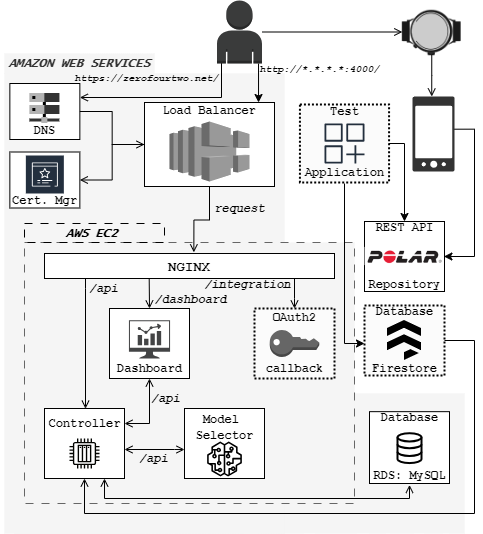
\includegraphics[width=0.9\textwidth]{images/sys_architecture.png}
    \caption{System Architecture.}
    \label{image:sys_architecture}
\end{figure}


\subsection{Web Services}
The various components that interact together to provide the system functionalities were developed and deployed in a loosely coupled manner and
interact with each other through RESTful API calls.  The Amazon Web Services (AWS) cloud platform was utilized as a Infrastructure as a Service (IaaS)
to provide the compute and storage resources required to run the various components with the EC2 Micro Virtual Machine, RDS (MySQL), 
Route 53 (Domain Naming Service), Elastic Load Balancer (ELB) and Software as a Service (Saas) for data storage with
Relational Database Service (RDS).

\subsubsection*{Domain Name} A domain name was registered on Route 53 and linked to the Elastic Load Balancer (ELB) to provide a consistent means of 
accessing the web application. IP addresses assigned to an instance of the EC2 Micro Virtual Machine are not static and will change each time the 
instance is restarted, this is guaranteed to break connection to the PolarFlow REST API and will require frequent modification of configuration files. 
Hence, request to the domain name is redirected to the ELB which in turn routes the request to the EC2 instance. A SSL/TLS security layer was added to 
the domain name to provide secure communication between the user and the web application as part of the requirements for the project. 

\subsubsection*{Controller} The Controller
\subsection{Database Design}
\begin{figure}[h!]
    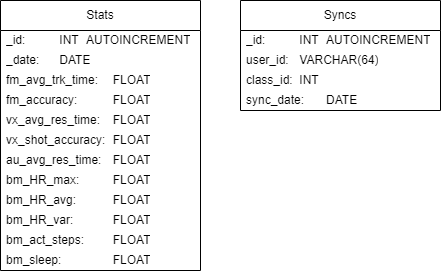
\includegraphics[width=0.9\textwidth]{images/db_schema.png}
    \caption{Database Design.}
    \label{image:databaseDesign}
\end{figure}


The machine learning services were developed using the 
sklearn library, Keras TensorFlow library and Flask web framework. The services were deployed on a cloud server to provide real-time best
model selection for users' performance prediction.

%Image \ref{image:sysArchitecture} can be referenced with the label given to the image, \\ i.e. \textbf{\textbackslash{}ref\{image:sysArchitecture\}}. 
Note that \LaTeX will place the image wherever it deems fit. Don't bother trying to change where a table or figure is placed until your document is ready for final layout.